\chapter{Description}

Vuistregel morfologisch effect lokale rivieringrepen

\section{Karakter van bodemverandering door rivieringrepen}

Een rivieringreep kan leiden tot veranderingen in het stroombeeld van het zomerbed.
De reaktie van de bodemligging in het zomerbed hierop is dan afhankelijk van de

\hspace{1cm}\emph{grootte, duur en lengteschaal van deze verandering in het zomerbed-stroombeeld.}

Het bepalen en karakteriseren van de veranderingen in het zomerbed-stroombeeld is dan ook de kern van de in dit memorandum afgeleide vuistregel.

Ter plekke van de herinrichting verlaat een deel van de afvoer het zomerbed (het deel tussen de normaallijnen), stroomt door de verruimde uiterwaard/nevengeul of oeverzone, en keert aan de benedenstroomse rand van het projectgebied weer terug in
het zomerbed.
De veranderingen in het stroombeeld wekken in het zomerbed aanzanding op bij de "splitsing" van de extra stroombaan uit het zomerbed en erosie bij de "samenvoeging" van de extra stroombaan naar zomerbed.
Omdat de rivierafvoer varieert, verandert ook dit patroon van aanzanding en erosie gedurende het seizoen.
Het gevolg hiervan is dat gedurende het jaar een deel van de bodemverandering blijft liggen en een deel stroomafwaarts verplaatst.
Dieptevermindering vindt dus niet alleen plaats ter plekke van de splitsende stroombaan, maar door het verplaatsende deel ook
stroomafwaarts ervan.

De bodemverandering door rivierverruiming kent grofweg de volgende karakteristieken:

\begin{itemize}
\item De grootte van de bodemverandering kent een seizoensvariatie; maximaal aan het einde van het hoogwaterseizoen en minimaal aan het einde van het laagwaterseizoen.

\item Door verplaatsing van een deel van de bodemverandering stroomafwaarts is het niet voldoende om alleen ter plekke van de rivierverruiming bodemveranderingen te beoordelen.

\item Het effect is maximaal aan de zijde van de ingreep.
\end{itemize}

Omdat een deel van de bodemveranderingen niet op de lokatie van de rivierverruiming blijft maar stroomafwaarts verplaatst, kunnen de morfologische effecten van benedenstroomse projecten worden versterkt.
Immers, in het geval van \'e\'en enkele rivierverruiming is de maximale bodemverandering aan het einde van het
hoogwaterseizoen het gevolg van de ontwikkeling tijdens het hoogwater.
Maar bij een serie ingrepen over een traject (bijvoorbeeld kribverlaging) kan de ontwikkeling tijdens hoogwater worden "geholpen" door de passerende bodemgolven, zodat een hogere eindwaarde wordt bereikt.
Met andere woorden, bij ingrepen over een langer traject kan de gecre\"eerde morfodynamiek tot grotere bodemveranderingen leiden dan bij
vergelijkbare maar ge\"isoleerde ingrepen.

Het bovenstaande leidt tot de volgende uitgangspunten.
De vuistregel die in dit memorandum wordt afgeleid

\begin{itemize}
\item heeft slechts betrekking op afzonderlijke effecten van lokale ingrepen die een lengte hebben van maximaal een enkele uiterwaard

\item neemt de seizoensvariatie in beschouwing

\item moet een indicatie geven van de ruimtelijke verdeling
\end{itemize}

\section{Karakterizering veranderingen in het zomerbed-stroombeeld}

Bijvoorbeeld bij rivierverruiming in de uiterwaard vindt zonder permanent meestromende nevengeulen de verandering in het zomerbedstroombeeld alleen plaats tijdens hoogwater.
Bij rivierverruiming met permanent meestromende nevengeulen en/of aangepaste oevers (kribverlaging) of bij hernormalisatie van het zomerbed verandert het zomerbed-stroombeeld ook voor gewone en lagere afvoeren.
Het is daarom van belang om het zomerbed-stroombeeld bij verschillende afvoerniveaus te bepalen.

Een voor de morfologie van het zomerbed belangrijke rivieringreep is de aanleg van nevengeulen.
De grootte van de nevengeulafvoer verloopt met de rivierafvoer.
Omdat de hydraulische parameters van de nevengeul in de loop van de tijd kunnen vari\"eren (begroeiing, aanzanding, erosie) wordt voor het regelen van de nevengeulafvoer gebruik gemaakt van afvoerregelwerken.
Een karakteristiek hiervan voor een overlaat (drempel) en onderlaat (duiker) is gegeven in \autoref{Fig1}.

\begin{figure}
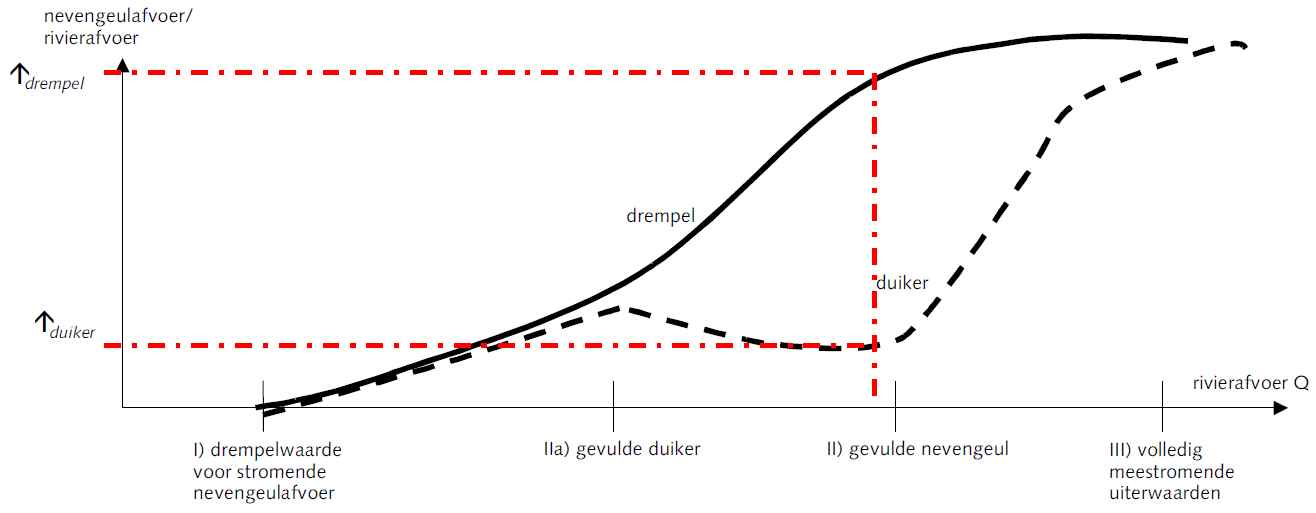
\includegraphics[width=\columnwidth]{figures/Fig1.png}
\caption{Schets van afvoerverloop door een nevengeul.}
\label{Fig1}
\end{figure}

Zoals \autoref{Fig1} weergeeft kent de nevengeulafvoer een aantal karakteristieke situaties die gemarkeerd worden met: i) het begin van stroming in de nevengeul; ii) de tot de oevers gevulde nevengeul en iii) ontwikkelde stroming in nevengeul en uiterwaard.
In geval van een duiker is er eventueel nog een karakteristiek afvoerniveau als de duiker volledig is gevuld.

Om de situatie bij hoogwater te kunnen karakteriseren is vervolgens onderscheid nuttig in een situatie waarin uiterwaarden beginnen mee te stromen, en een situatie met goed ontwikkelde stroming in de uiterwaarden.
Volgens \autoref{Fig2a} kan de grens voor beide situaties worden gelegd bij een Bovenrijnafvoer van 6.000 m\textsuperscript{3}/s.
Ook voor de oeverzone (\autoref{Fig2b}) geldt dat de afvoer grofweg ontwikkeld is voor Bovenrijnafvoeren groter dan
6.000 m\textsuperscript{3}/s.

\begin{figure}
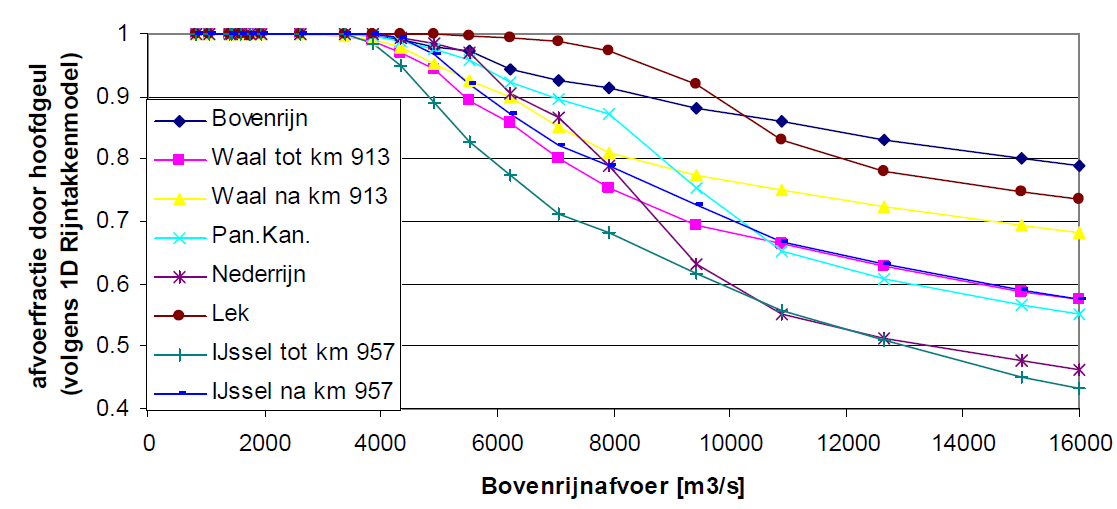
\includegraphics[width=\columnwidth]{figures/Fig2a.png}
\caption{Trajectgemiddelde relatieve afvoerfractie door de hoofdgeul (1D Rijntakkenmodel).}
\label{Fig2a}
\end{figure}

\begin{figure}
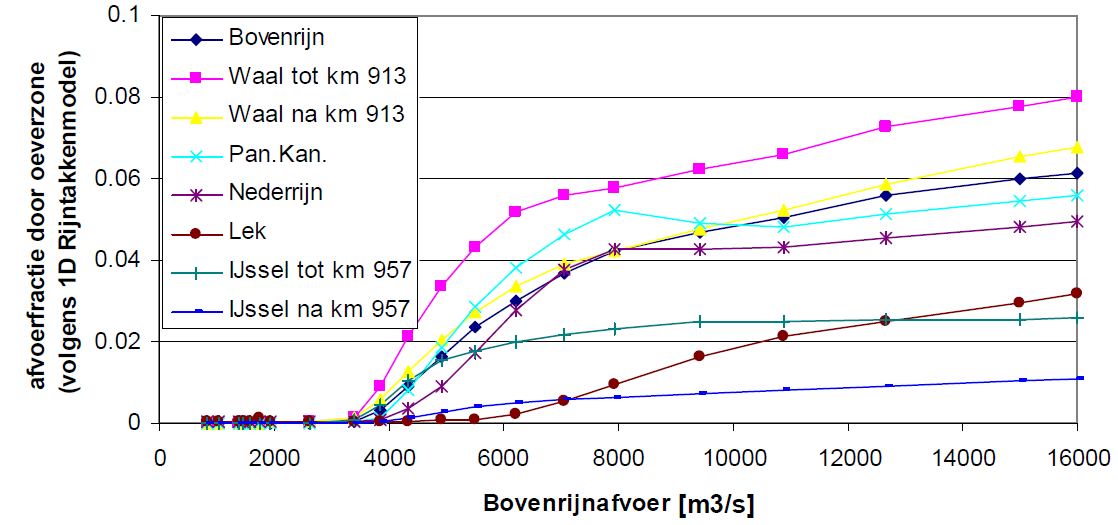
\includegraphics[width=\columnwidth]{figures/Fig2b.png}
\caption{Trajectgemiddelde relatieve afvoerfractie door de oeverzone (1D Rijntakkenmodel).}
\label{Fig2b}
\end{figure}

Om een hydrograaf passend te schematiseren kunnen deze karakteristieke waarden worden gebruikt om discrete afvoerblokken te onderscheiden.
Zoals uit \autoref{Tab1} blijkt zijn drie blokken daarbij voldoende voor een groot aantal maatregelen.
Daarom wordt gesteld dat \emph{het schematiseren van het jaarlijkse afvoerverloop in drie blokken generiek genoeg is voor de effectbepaling}.

\begin{table}
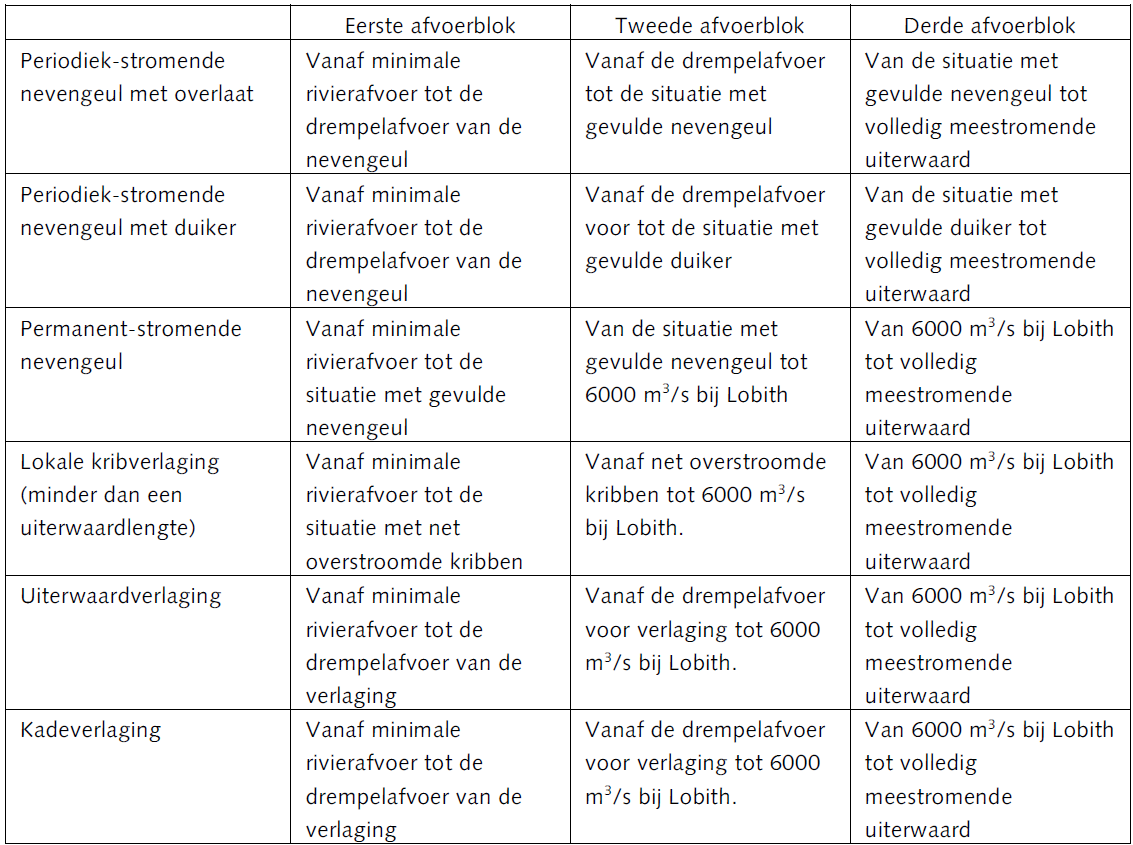
\includegraphics[width=\columnwidth]{figures/Tab1a.png}
\caption{Overzicht afvoerblokken voor verschillende ingrepen bij een vrij-afstromende Rijntak.}
\label{Tab1}
\end{table}

Voor een rivier die gedurende een periode $T_\text{stuw}$ wordt gestuwd geldt dat de minimale rivierafvoer wordt afgestemd op het afvoerniveau dat de stuwen worden getrokken.
Voor de Nederrijn geldt volgens \autoref{Fig6} dat de stuwen grofweg worden getrokken bij een Bovenrijnafvoer van 1500 m\textsuperscript{3}/s (gedurende 57 \% van het jaar overschreden), en dat de tak min of meer vrij afstromend is voor Bovenrijnafvoeren groter dan 2200 m\textsuperscript{3}/s (gedurende 33 \% van het jaar).

\begin{table}
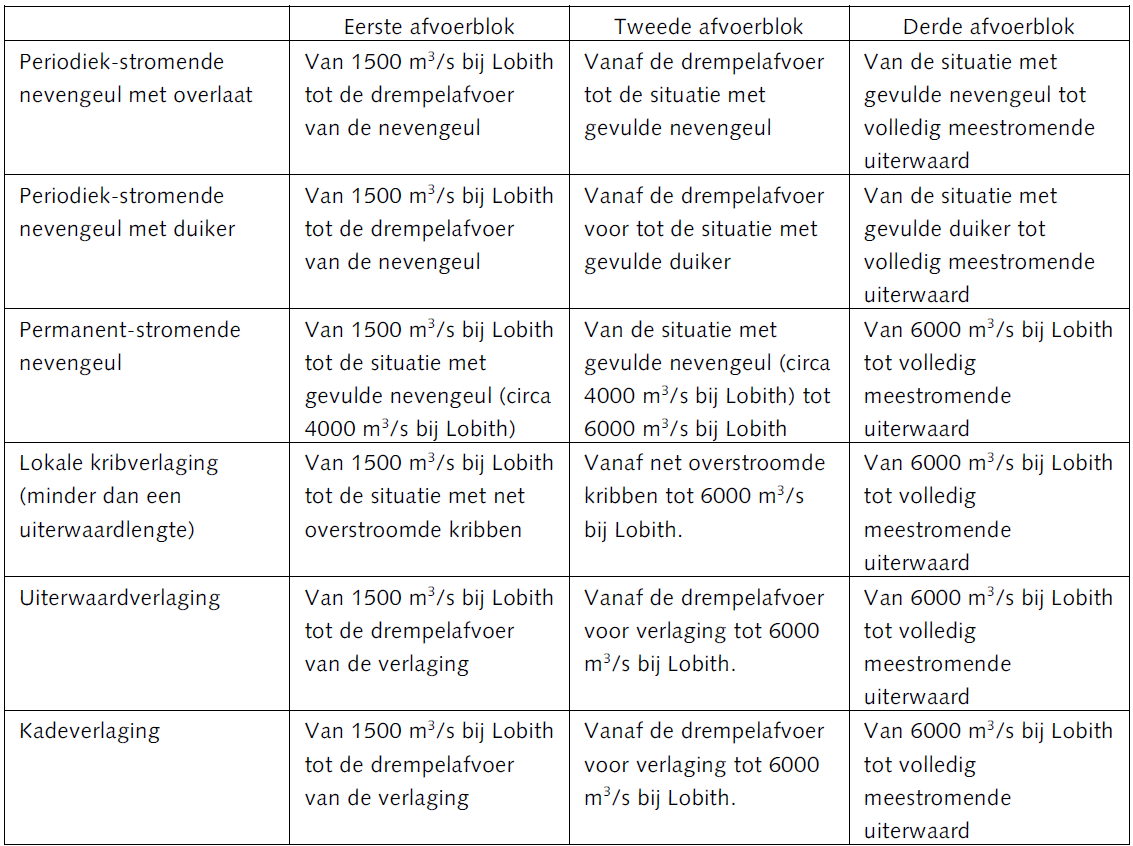
\includegraphics[width=\columnwidth]{figures/Tab1b.png}
\caption{Overzicht afvoerblokken voor verschillende ingrepen bij de Nederrijn.}
\label{Tab2}
\end{table}

\begin{table}
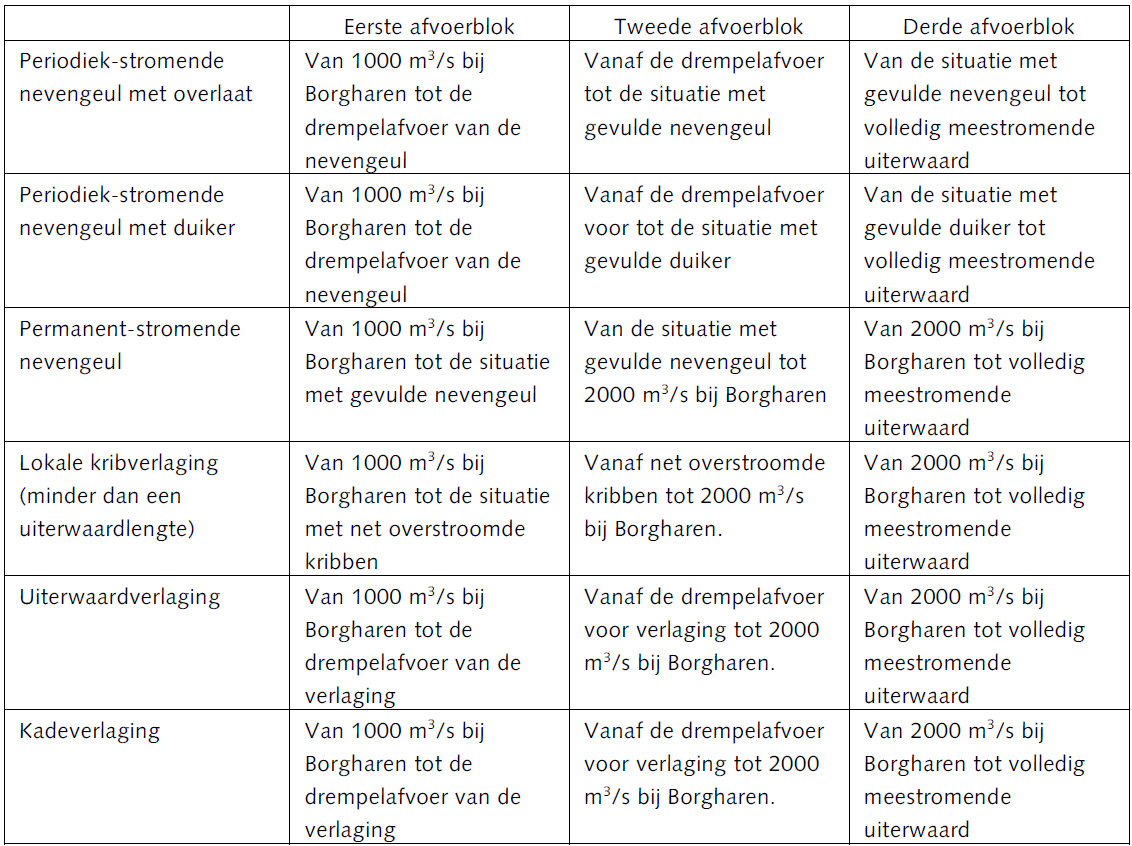
\includegraphics[width=\columnwidth]{figures/Tab1c.png}
\caption{Overzicht afvoerblokken voor verschillende ingrepen bij de Maas.}
\label{Tab3}
\end{table}

\begin{figure}
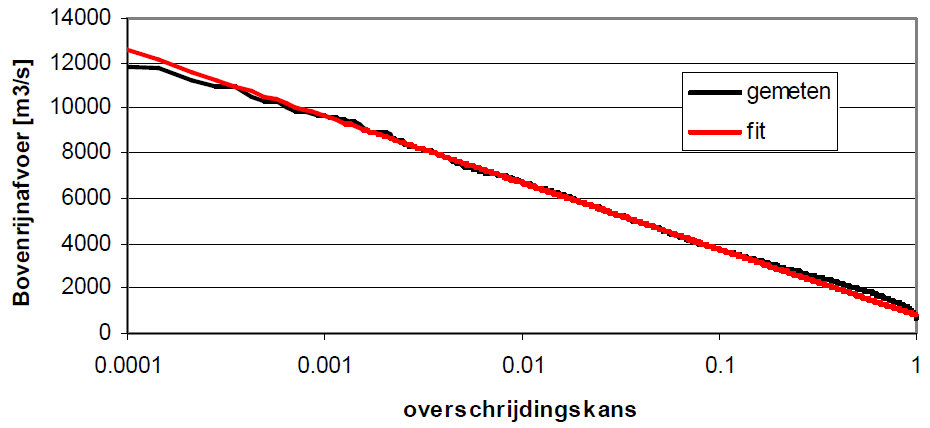
\includegraphics[width=\columnwidth]{figures/Fig3a.png}
\caption{Overschrijdingskromme van Bovenrijnafvoeren (1970-2000).}
\label{Fig3a}
\end{figure}

\begin{figure}
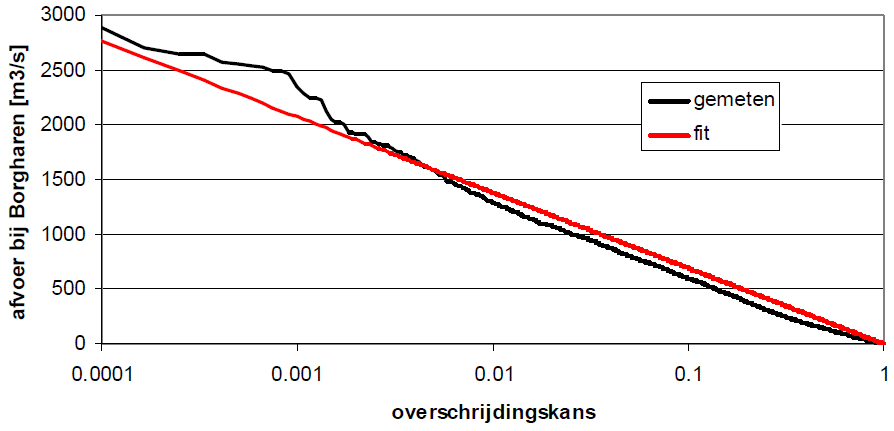
\includegraphics[width=\columnwidth]{figures/Fig3b.png}
\caption{Overschrijdingskromme van Maasafvoeren bij Borgharen (1975-2007).}
\label{Fig3b}
\end{figure}

Om de jaarlijkse overschrijdingsperiode van Bovenrijnafvoeren snel te kunnen schatten kan een functie worden gebruikt die is gefit op gemeten waarden uit de periode 1970-2000 (\autoref{Fig3a}).
Het aantal dagen dat een Bovenrijnafvoer $Q_\text{Bovenrijn}$ wordt overschreden is dan
%
\begin{equation}
\label{Eq1a}
T_\text{overschrijdingsperiode} = 365 e^{\left ( \frac{800 -  Q_\text{Bovenrijn}}{1280} \right )}
\end{equation}

Voor de Maas, waar door afpleistering (Grensmaas) en stuwen (Zandmaas) met name de hogere afvoeren van belang zijn voor de morfologie, kan de gemiddelde overschrijdingsperiode van de afvoer bij Borgharen worden geschat met
%
\begin{equation}
\label{Eq1b}
T_\text{overschrijdingsperiode} = 365 e^{\left ( \frac{-  Q_\text{Borgharen}}{300} \right )}
\end{equation}

\section{Achtergrond relaxatie model voor morfologische veranderingen}

Om een eerste inschatting van morfologische effecten in het zomerbed te kunnen maken wordt een vuistregel afgeleid op basis van een zeer vereenvoudigd model.
Dit model en de afleiding van de vuistregel wordt hier beknopt beschreven.
Veronderstel een quasi-stationaire stroming en een onttrekking van afvoer en sediment uit een stroombaan, waarbij de lokale waterspiegel onafhankelijk is van de hydraulische en morfologische veranderingen in de hoofdgeul (\emph{rigid-lid} benadering).

\begin{figure}
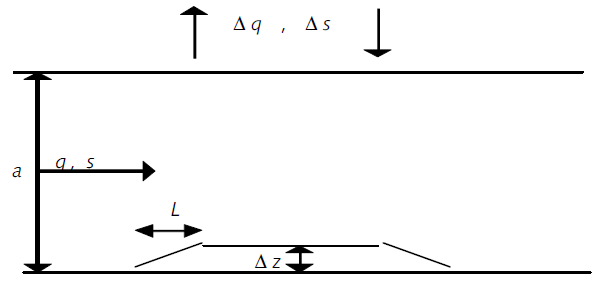
\includegraphics[width=\columnwidth]{figures/Fig4.png}
\caption{Principeschets afvoer en sedimentonttrekking}
\label{Fig4}
\end{figure}

De reactie van het zomerbed wordt hier voorgesteld met een bodemverandering $\Delta z$ \unitbrackets{m} (bodemsprong of bodemverval) die klein is ten opzichte van de diepte.
Voor zowel het water als het sediment kan een massabalans voor de stroombaan door de hoofdgeul worden opgesteld;

\begin{tabular}{p{3cm}p{\textwidth-3cm}}
water & \parbox{\textwidth-4cm}{\begin{equation}
\pdiff{q_\text{hg}}{s} = -q_\text{uit}
\end{equation}} \label{Eq2} \\
sedimentbalans & \parbox{\textwidth-4cm}{\begin{equation}
\pdiff{z}{t} + \pdiff{s_\text{hg}}{s}= -q_\text{uit} = -s_\text{uit}
\end{equation}} \label{Eq3} \\
\end{tabular}

waarin

\begin{symbollist}
\item[$a$] \unitbrackets{m} diepte in de hoofdgeul
\item[$q_\text{hg}$] \unitbrackets{m\textsuperscript{2}/s} afvoer door hoofdgeul per eenheid van breedte (specifieke afvoer)
\item[$q_\text{uit}$] \unitbrackets{m\textsuperscript{2}/ms} \emph{onttrokken specifieke} afvoer \emph{naar} de uiterwaard per eenheid van
lengte
\item[$s$] \unitbrackets{m} co\"ordinaat in stroomrichting
\item[$u$] \unitbrackets{m/s} snelheid
\item[$z$] \unitbrackets{m} bodemverandering door herinrichting
\item[$s_\text{hg}$] \unitbrackets{m\textsuperscript{2}/s} specifiek sedimenttransport door hoofdgeul per eenheid van breedte
\item[$s_\text{uit}$] \unitbrackets{m\textsuperscript{2}/ms} \emph{onttrokken specifiek} sedimenttransport \emph{naar} de uiterwaard per eenheid van lengte
\end{symbollist}

De specifieke transportcapaciteit in de hoofdgeul, $s_\text{hg}$, wordt benaderd met $s_\text{hg} = m \left ( \frac{h_\text{hg}}{a} \right )^b$ met $b$ van de orde 5 (Engelund en Hansen, 1967).
Gradi\"enten in transportcapaciteit worden dan geschreven als
%
\begin{equation}
\pdiff{s_\text{hg}}{s} \approx b \frac{s_\text{hg}}{q_\text{hg}} \pdiff{q_\text{hg}}{s} + b \frac{s_\text{hg}}{a} \pdiff{z}{s}
\label{Eq4}
\end{equation}

Invullen van \autoref{Eq4} in \autoref{Eq2} en \autoref{Eq3}, de massabalansen voor water en sediment levert dan
%
\begin{equation}
\frac{a}{b s_\text{hg}} \pdiff{z}{t} + \pdiff{z}{s} = a \frac{q_\text{uit}}{q_\text{hg}} - a \frac{s_\text{uit}}{b s_\text{hg}}
\label{Eq5}
\end{equation}

De dynamische bodemveranderingen worden aan de bovenstroomse zijde van de maatregel opgebouwd.
De lengte $L$ waarover dit gebeurt, komt overeen met het traject waarin de afvoer uit de hoofdgeul verdwijnt en waarin het stroombeeld in de hoofdgeul aan deze verminderde afvoer is aangepast.
Deze lengte $L$ is dus \emph{niet} per definitie de lengte van de maatregel of de afstand tussen in- en uitstroomopening van een
nevengeul.
Integratie van \autoref{Eq5} over deze afstand $L$ levert dan een relaxatiemodel voor de dynamische bodemverandering ten gevolge van herinrichting $\diff{\Delta z}{t} = \frac{\Delta z_e - \Delta z}{T}$ met een morfologische tijdschaal $T \approx \frac{a L}{bs_\text{hg}}$ en een evenwichtsbodemverandering
%
\begin{equation}
\Delta z_e = -a \left ( \frac{\Delta q_\text{hg}}{q_\text{hg}} + \frac{\Delta s_\text{hg}}{b s_\text{hg}} \right )
\label{Eq6}
\end{equation}

Het relaxatiegedrag volgens \autoref{Eq5} kan ook worden gevonden in numerieke modellen (zowel 1D als 2D).

Voor de afleiding van de vuistregel wordt gesteld dat de bodemverandering $\Delta z$ kan worden opgevat als de bodemverandering door een ingreep, op een afstand $L$ langs een lijn loodrecht op de stroombanen aan de bovenstroomse rand van de ingreep.
De evenwichtswaarde $\Delta z_e$ is volgens \autoref{Eq6} afhankelijk van de oorspronkelijke waterdiepte, de relatieve verandering in specifieke afvoer en de relatieve verandering in sediment transport.
Deze laatste term is de bijdrage van sedimentonttrekking naar de nevengeul die het effect van de verminderde hoofdgeulafvoer dempt.
Verwaarlozing van deze relatief kleine dempende bijdrage leidt tot een conservatieve benadering.
Voor de korte inrichtingsprojecten waar de vuistregel voor geldt zijn waterstandsveranderingen een orde kleiner dan bodemveranderingen, daarom kan met \autoref{Eq6} worden gesteld dat de evenwichtswaarde van bodemveranderingen $\Delta z_e$ gelijk is aan het produkt van waterdiepte en relatieve snelheids- of afvoerverandering.

Ook voor bodemmateriaal met varierende korrelgrootte (zand en grind) kan een benaderend model worden afgeleid, als wordt aangenomen dat de mobiliteit van de verschillende fracties onderling niet wordt be\"invloed (Bijlage C uit WD nota Kennis en instrumenten Maas morfologie).
Een dergelijke aanname is geldig bij voldoende hoge bodemschuifspanningen, zoals tijdens hoogwater.

\section{Toepassing relaxatiemodel voor seizoenseffecten}

Veronderstel dat de bodemligging in een periode met een relaxatiegedrag (als oplossing van model \autoref{Eq6}) kan worden voorspeld volgens
%
\begin{equation}
z_i = z_i (0) + [z_{ie} - z_i(0)](1 - e^{-t/T_{mi}})
\label{Eq7}
\end{equation}

met

\begin{symbollist}
\item[$z_i$] \unitbrackets{m} het morfologisch effect van ingrepen gedurende periode $i$
\item[$z_i(0)$] \unitbrackets{m} het morfologisch effect van ingrepen bij aanvang van periode $i$
\item[$z_{ie}$] \unitbrackets{m} de evenwichtswaarde van het morfologisch effect in periode $i$
\item[$T_{mi}$] \unitbrackets{dg} de morfologische tijdschaal gedurende periode $i$
\end{symbollist}

\begin{figure}
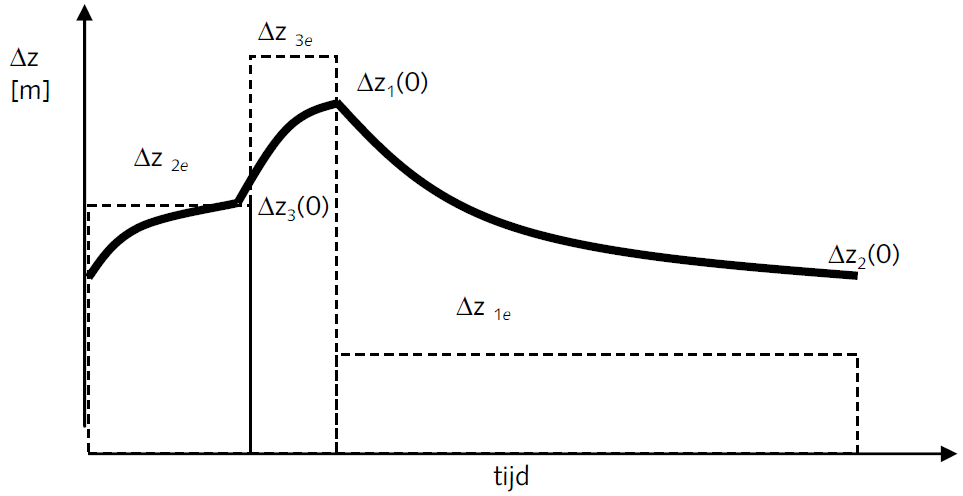
\includegraphics[width=\columnwidth]{figures/Fig5.png}
\caption{Schets van maximale bodemveranderingen op de bovenrand.}
\label{Fig5}
\end{figure}

Aan het einde van een periode met index $i$ is volgens \autoref{Eq7} het morfologisch effect bepaald met
%
\begin{equation}
z_{i+1}(0) = z_i (0) \sigma_i + z_{ie} (1-\sigma_i) \text{ met } \sigma_i = e^{-T_i/T_{mi}}
\autoref{Eq8a}
\end{equation}

Als het jaarlijks verloop wordt weergegeven met drie perioden, dan kan voor elk van deze perioden worden gesteld
%
\begin{align}
z_2(0) &= z_1 (0) \sigma_1 + z_{1e} (1-\sigma_1) \label{Eq8b} \\
z_3(0) &= z_2 (0) \sigma_2 + z_{2e} (1-\sigma_2) \label{Eq8c} \\
z_1(0) &= z_3 (0) \sigma_3 + z_{3e} (1-\sigma_3) \label{Eq8d}
\end{align}

Hiermee kan voor de karakteristieke bodemveranderingen worden gevonden
%
\begin{align}
z_1(0) &= \frac{z_{1e} (1-\sigma_1) \sigma_2 \sigma_3 + z_{2e} (1-\sigma_2) \sigma_3 + z_{3e} (1-\sigma_3)}{1 - \sigma_1 \sigma_2 \sigma_3} \label{Eq8e} \\
z_2(0) &= \frac{z_{1e} (1-\sigma_1) + z_{2e} (1-\sigma_2) \sigma_3 \sigma_1 + z_{3e} (1-\sigma_3) \sigma_1}{1 - \sigma_1 \sigma_2 \sigma_3} \label{Eq8f} \\
z_3(0) &= \frac{z_{1e} (1-\sigma_1) \sigma_2 + z_{2e} (1-\sigma_2) + z_{3e} (1-\sigma_3) \sigma_1 \sigma_2}{1 - \sigma_1 \sigma_2 \sigma_3} \label{Eq8g}
\end{align}

Een ondergrens voor het morfologisch effect van ingrepen is dan $\min[z_1(0), z_2(0), z_3(0)]$ en een bovengrens wordt gegeven door $\max[z_1(0), z_2(0), z_3(0)]$.
Met een verloop zoals is weergegeven in \autoref{Fig5} is de bodemverandering
\begin{itemize}
\item maximaal met $z_1(0)$ (\autoref{Eq8e}) na de hoogwaterperiode 3 (het derde afvoerblok uit \autoref{Tab2})
\item minimaal met $z_2(0)$ (\autoref{Eq8f}) na de laagwaterperiode 1 (het eerste afvoerblok uit \autoref{Tab2}).
\end{itemize}

De invloed van stuwprogramma's kan bijvoorbeed worden gesimuleerd door tussen het hoogwaterblok 3 en het laagwaterblok 1 een jaarlijkse periode te introduceren zonder bodemveranderingen.

Behalve beide extremen kan een indruk worden gekregen van de jaargemiddelde bodemverandering door integratie van \autoref{Eq7} tot
%
\begin{equation}
\bar{z} = \frac{\sum{z_{ie} t_i}}{\sum{t_i}} + \frac{\sum{(z_{ie}-z_i(0)) T_{mi} (\sigma_i-1)}}{\sum{t_i}}
\label{Eq8h}
\end{equation}

Als alle bodemveranderingen na het hoogwater worden weggebaggerd kan tenslotte een indruk worden verkregen van het jaarlijkse baggerbezwaar bij gebrek aan overdiepte.
Immers, met $z_1(0)=0$ door het baggeren is de maximale bodemverandering aan het einde van het hoogwaterseizoen met \autoref{Eq8a} tot \autoref{Eq8i} uit te schrijven tot het maximale baggerbezwaar
%
\begin{equation}
z_\text{mbb} = z_{1e}(1-\sigma_1) \sigma_2 \sigma_3 + z_{2e} (1-\sigma_2) \sigma_3 + z_{3w} (1-\sigma_3)
\label{Eq8i}
\end{equation}

Omdat in deze voorspelling geen rekening wordt gehouden met het sedimentaanbod van de rivier (zandvracht) kan \autoref{Eq8i} leiden tot een overschatting van de onderhoudslast.
\autoref{Eq8i} wordt dan ook niet verder uitgewerkt.

\section{Benadering ruimtelijk karakter van bodemverandering}

Met \autoref{Eq8e} is de maximale, en met \autoref{Eq8f} is de minimale bodemverandering aan de bovenstroomse rand van de ingreep vastgelegd.
In de stroombaan benedenstrooms hiervan bestaat de bodemverandering uit een minimale bodemverandering $z_{1e}$ plus het deel van de hoogwateraanzanding aan de bovenstroomse rand dat tijdens laagwater stroomafwaarts verplaatst.
Gedurende een hoogwater kan dit stroomafwaarts verplaatsend aanzandingsvolume zelfs leiden tot bodemveranderingen die tijdelijk groter
zijn dan $z_{2e}$ maar erg waarschijnlijk is dit niet.
Gemakshalve wordt daarom gesteld de maximale en minimale bodemverandering volgens \autoref{Eq8e} en \autoref{Eq8f} \emph{voor elk punt in het zomerbed ter hoogte van de ingreep} geldt.

Deze benadering houdt in dat op eerst elk WAQUA rekenpunt in het zomerbed een waarde $z_{1e}$, $z_{2e}$ en $z_{3e}$ kan worden bepaald.
Vervolgens kan met een geschatte waarde van $\sigma_1$, $\sigma_2$ en $\sigma_3$ met Verg.7-e en 7-f een inschatting voor de WAQUA rekenpunten maximale bodemverandering (aan het einde van het hoogwaterseizoen) worden gemaakt.

\section{Definitie tijdschalen voor bodemverandering}

De grootte van de maximale bodemverandering aan het einde van het hoogwaterseizoen en de minimale bodemverandering aan het einde van het
laagwaterseizoen is afhankelijk van de morfologische tijdschaal $T$ \unitbrackets{dg} die de reactietijd van de bodemligging beschrijft.
Deze tijdsschaal $T$ kan met de definitie van Verg.5 ook worden geschreven als $T=L/w$ met $w$ een voortplantingssnelheid van bodemveranderingen en $L$ de lengte langs een stroombaan waarover de bodemveranderingen worden opgebouwd.
Zoals eerder is opgemerkt komt deze lengte $L$ overeen met het traject waarin de afvoer uit de hoofdgeul verdwijnt en waarin het
stroombeeld in de hoofdgeul aan deze verminderde afvoer is aangepast.
Deze afstand varieert echter per stroombaan en per afvoersituatie.
Voor een eenduidig gebruik van de vuistregel wordt desondanks gemakshalve verondersteld dat deze lengte $L$ overeenkomt met tweemaal de hoofdgeulbreedte $B_\text{hoofdgeul}$.

De tweede parameter in de morfologische tijdschaal is de voortplantingssnelheid van bodemveranderingen.
Op basis van de statistiek van breedte-gemiddelde km-waarden van jaargemiddelde bodempeilingen (RIZA werkdoc.2005.044x) zijn hiervan
jaargemiddelde waarden bepaald.
Deze zijn in \autoref{Tab2} en \autoref{Tab3} weergegeven.

\begin{table}
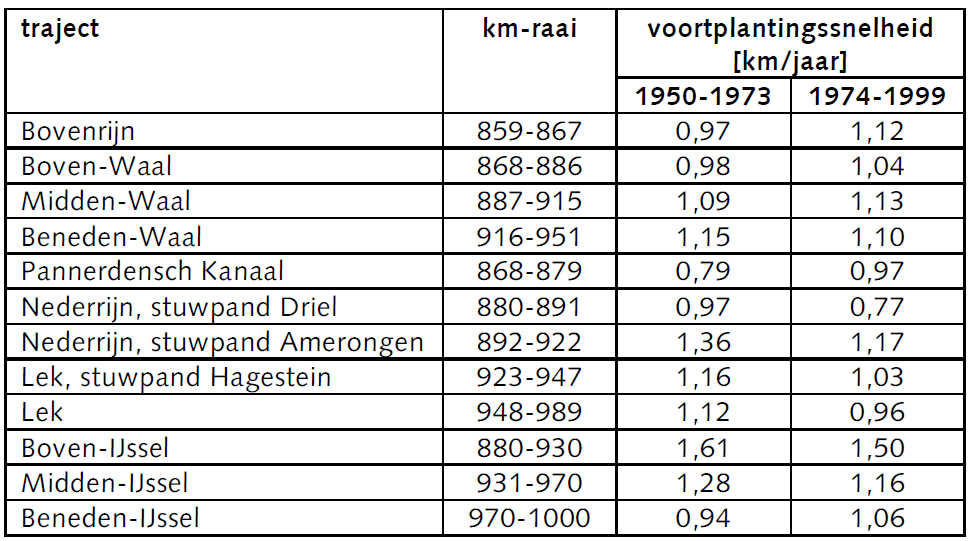
\includegraphics[width=\columnwidth]{figures/Tab2.png}
\caption{Overzicht gemiddelde voortplantingssnelheden (gebaseerd op km-gemiddelde bodemliggingen en inclusief de invloed van baggeren) RIZA werkdoc 2005.044x.}
\label{Tab2Again}
\end{table}

\begin{table}
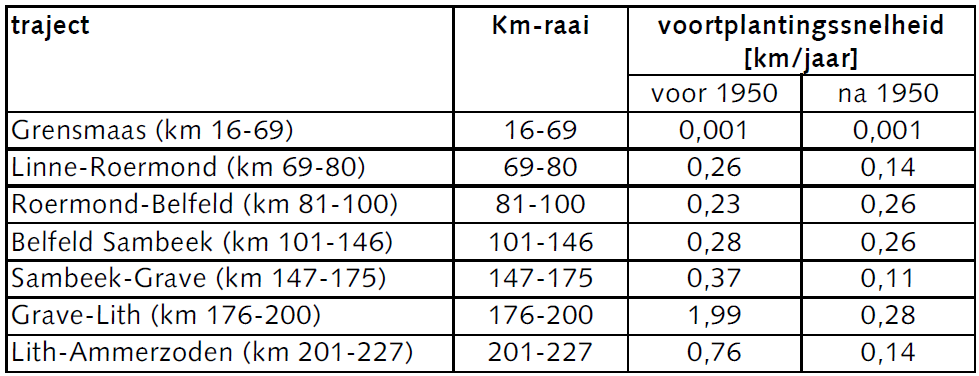
\includegraphics[width=\columnwidth]{figures/Tab3.png}
\caption{Overzicht trajectgemiddelde voortplantingssnelheden (gebaseerd op kmgemiddelde bodemliggingen en inclusief de invloed van baggeren) WD rapport Kennis en instrumenten Maas morfologie Inventarisatie behoefte monitoring en voorspelgereedschap)}
\label{Tab3Again}
\end{table}

\begin{table}
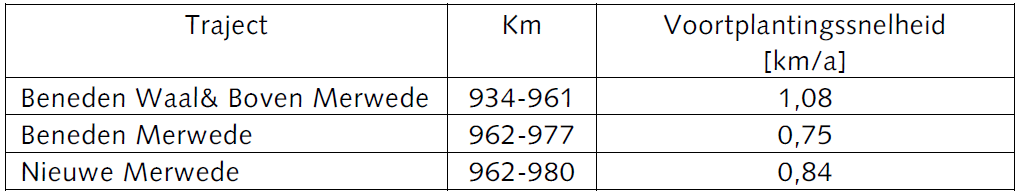
\includegraphics[width=\columnwidth]{figures/Tab4.png}
\caption{Overzicht trajectgemiddelde voortplantingssnelheden (gebaseerd op kmgemiddelde bodemliggingen uit de periode 1975-2000 inclusief de invloed van baggeren) RIZA WSR memo 2007-013 calibratie parameters Merwede.}
\label{Tab4}
\end{table}

Om deze empirische jaargemiddelde waarden te kunnen vertalen naar discrete waarden per afvoerblok wordt voor de vrij afstromende riviertakken de volgende benadering gebruikt.
Voor afvoerblokken met Bovenrijnafvoeren die overwegend groter zijn dan 4.000 m\textsuperscript{3}/s (gedurende gemiddeld 8 \% van het jaar) wordt een "hoogwatervoortplantingsnelheid" $w_h$ van 10 m/dag (3,65 km/jaar) gebruikt.

Voor de afvoerblokken met Bovenrijnafvoeren die overwegend lager zijn dan 4.000 m\textsuperscript{3}/s wordt een "laagwatervoortplantingssnelheid" $w_l$ gebruikt die is berekend met de jaargemiddelde waarde $\bar{w}$ volgens
%
\begin{equation}
w_l = \frac{\bar{w} - 0,082 \cdot 365}{0,918}
\label{Eq9}
\end{equation}

De benadering met \autoref{Eq9} geldt echter alleen voor de vrijstromende Rijntakken, en dus bijvoorbeeld niet voor de Nederrijn, waar bij lage Bovenrijnafvoeren de stuwen gesloten blijven (\autoref{Fig6}).

\begin{figure}
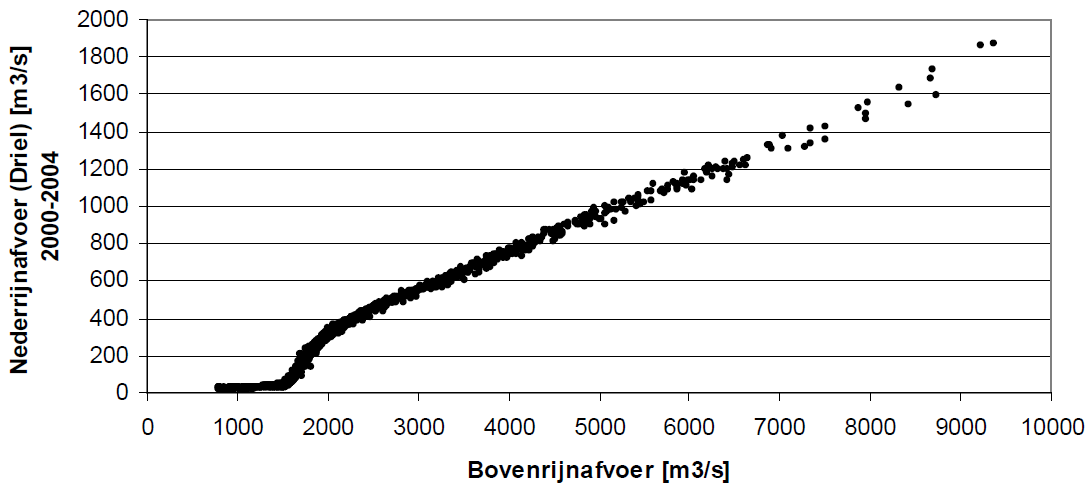
\includegraphics[width=\columnwidth]{figures/Fig6.png}
\caption{Nederrijn afvoeren (Driel-boven) volgens Donar in de periode 2000-2004).}
\label{Fig6}
\end{figure}

Voor de Nederrijn geldt volgens \autoref{Fig6} dat de stuwen grofweg worden getrokken bij een Bovenrijnafvoer van 1500 m\textsuperscript{3}/s (57 \% van het jaar overschreden), en dat de tak min of meer vrij afstromend is voor Bovenrijnafvoeren groter dan 2200 m\textsuperscript{3}/s (gedurende 33 \% van het jaar). Voor de karakteristieke laagwatervoortplantingssnelheid wordt daarom verondersteld $\bar{w} = 0,082 w_h + (0,918 - 0,33) w_l$ zodat met $w_h = 3,65$ km/jaar wordt gevonden
%
\begin{equation}
w_l = \frac{\bar{w} - 0,082 \cdot 3,65}{0,918 - 0,33}
\label{Eq10a}
\end{equation}

Voor de Maas wordt de volgende benadering toegepast.
Aangenomen wordt dat de Maasstuwen gemiddeld 10 dagen per jaar (3 \% van de tijd) getrokken zijn, zodat de verplaatsingsnelheid kan worden geschat met
%
\begin{equation}
w_h = \frac{\bar{w}}{0,03}
\label{10b}
\end{equation}


Voor de Grensmaas tenslotte, geldt dat de pleisterlaag op de rivierbodem pas bij afvoeren groter dan 1000 m\textsuperscript{3}/s, gemiddeld gedurende 4 dagen per jaar, mobiel wordt.
De verplaatsingsnelheid wordt dan geschat met
%
\begin{equation}
w_h = \frac{\bar{w}}{0,01}
\label{Eq10c}
\end{equation}

Met de benaderingen van \autoref{Eq9} tot \autoref{Eq10c} en de jaargemiddelde waarden uit \autoref{Tab2} en \autoref{Tab3} wordt een schatting gevonden van de voortplantingssnelheden tijdens het hoog- en laagwaterseizoen.

\begin{table}
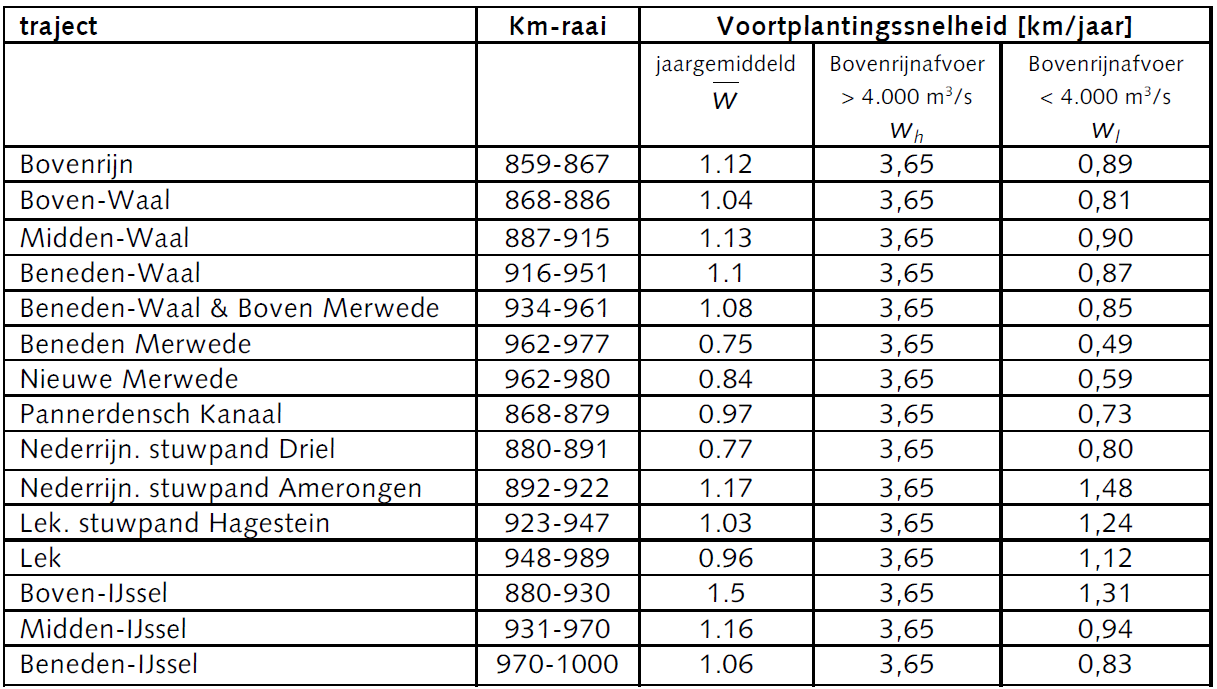
\includegraphics[width=\columnwidth]{figures/Tab4_the2nd.png}
\caption{Representatieve voortplantingssnelheden hoog- en laagwaterafvoeren Rijntakken.}
\label{Tab4RT}
\end{table}

\begin{table}
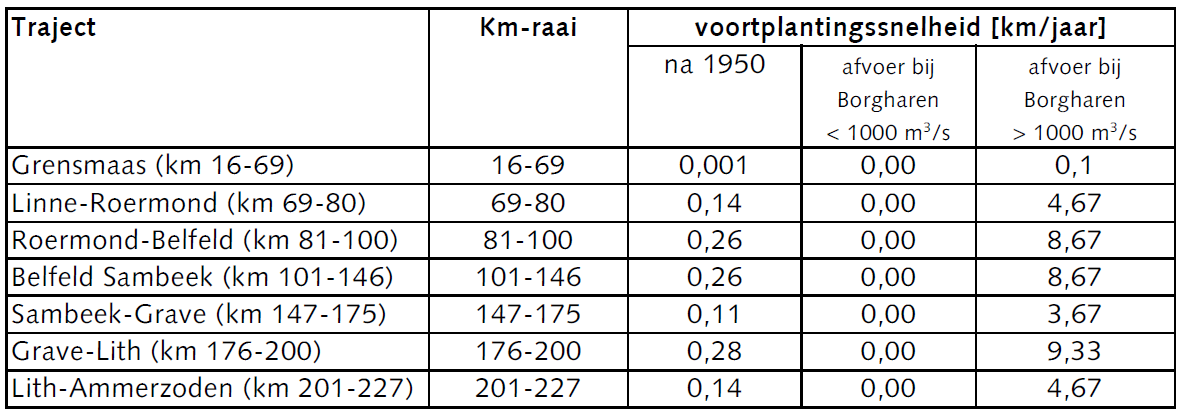
\includegraphics[width=\columnwidth]{figures/Tab5.png}
\caption{Representatieve voortplantingssnelheden hoog- en laagwaterafvoeren Maas.}
\label{Tab5}
\end{table}

\section{Stappenplan voor de opbouw van de WAQUA vuistregel}

\begin{enumerate}
\item Karakteriseer maatregel

\begin{itemize}
\item Bepaal drempelafvoer $Q_\text{dr}$ (bij Lobith/Borgharen) waarbij de maatregel effectief via hydraulica het zomerbed-stroombeeld begint te be\"invloeden.

\item Bepaal $Q_\text{bv}$ (bij Lobith/Borgharen) waarbij de maatregel tot aan de rand stroomvoerend (bankvullend) is
\end{itemize}

\item Definieer afvoerblokken (blok 1 "laagwater", blok 3 "hoogwater" en blok 2 "overgang tussen laag- en hoogwater") volgens

\begin{itemize}
\item \autoref{Tab7} voor de vrij afstromende Rijntakken
\item \autoref{Tab8} voor de Nederrijn en Lek
\item \autoref{Tab9} voor de Maas
\end{itemize}

\item Bereken karakteristieke bodemverandering per rekenpunt in het zomerbed

\begin{itemize}
\item maximale waarde \unitbrackets{m} aan het einde van het hoogwaterseizoen
%
\begin{equation}
z_1(0) = \frac{z_{1e} (1-\sigma_1) \sigma_2 \sigma_3 + z_{2e} (1-\sigma_2) \sigma_3 + z_{3e} (1-\sigma_3)}{1 - \sigma_1 \sigma_2 \sigma_3}
\end{equation}
\item minimale waarde \unitbrackets{m} aan het einde van het laagwaterseizoen
%
\begin{equation}
z_2(0) = \frac{z_{1e} (1-\sigma_1) + z_{2e} (1-\sigma_2) \sigma_3 \sigma_1 + z_{3e} (1-\sigma_3) \sigma_1}{1 - \sigma_1 \sigma_2 \sigma_3}
\end{equation}
\item tussenwaarde \unitbrackets{m} aan het einde van de overgang van laag- naar hoogwater
%
\begin{equation}
z_3(0) = \frac{z_{1e} (1-\sigma_1) \sigma_2 + z_{2e} (1-\sigma_2) + z_{3e} (1-\sigma_3) \sigma_1 \sigma_2}{1 - \sigma_1 \sigma_2 \sigma_3}
\end{equation}
\item jaargemiddelde waarde \unitbrackets{m}
%
\begin{equation}
z_m = T_1 z_1(0) + T_2 z_2(0) + T_3 z_3(0)
\end{equation}
\item een maximaal jaarlijks baggerbezwaar (zonder rekening te houden met overdiepten)
%
\begin{equation}
z_\text{mbb} = z_{1e} (1-\sigma_1) \sigma_2 \sigma_3 + z_{2e} (1-\sigma_2) \sigma_3 + z_{3e} (1-\sigma_3)
\end{equation}
\end{itemize}

\end{enumerate}

\section{Plot de relevante karakteristieke bodemveranderingen in kleurklassen op een kaart}

\begin{table}
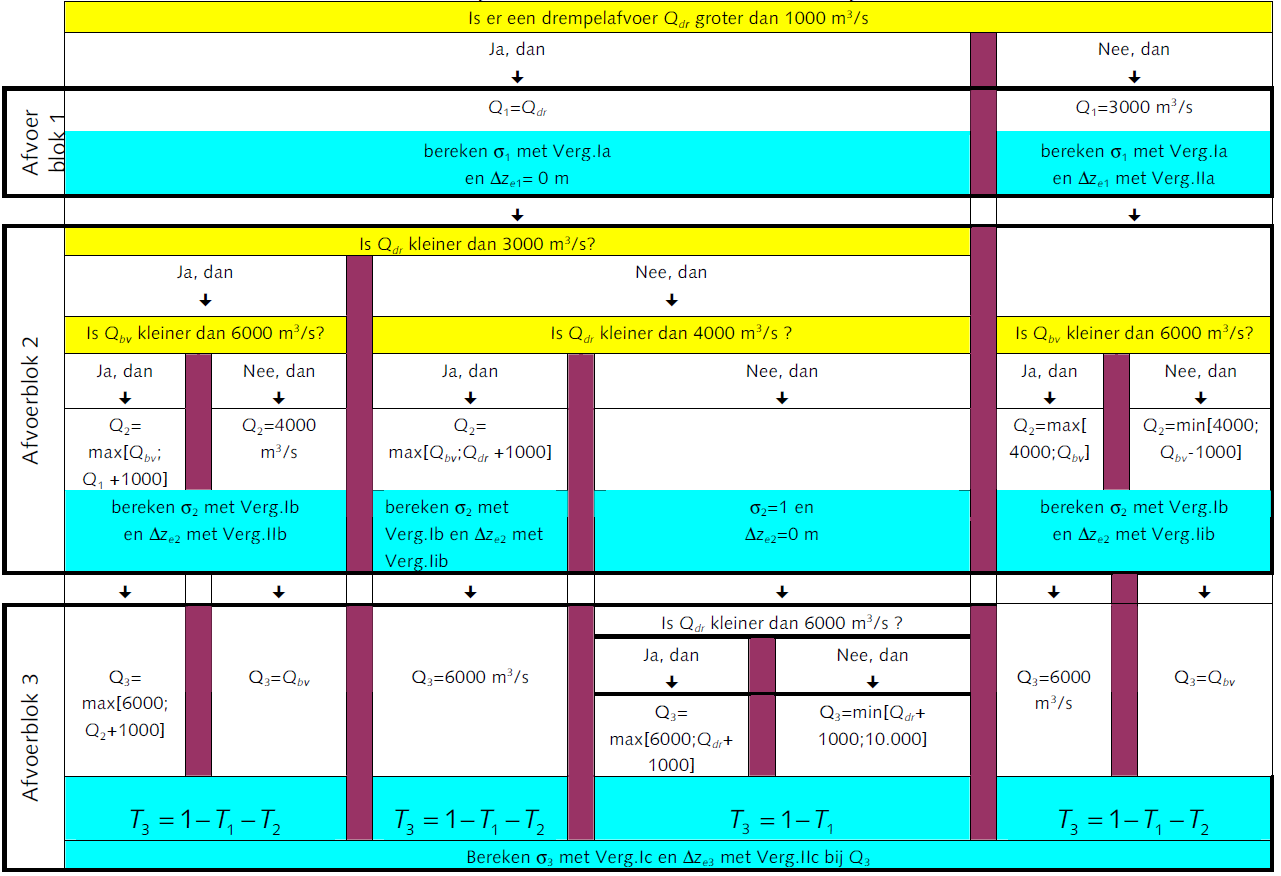
\includegraphics[width=\columnwidth]{figures/Tab7.png}
\caption{Hoofdlijn definitie afvoerblokken voor de Rijntakken}
\label{Tab7}
\end{table}

\begin{equation}
\sigma_1 = e^{-\frac{w_l}{2 B_n} T_1}
\end{equation}
met $T_1 = e^{\left ( \frac{800-Q_\text{stuw}}{1280} \right )} - e^{\left ( \frac{800-Q_1}{1280} \right )}$ en $w_l$ uit \autoref{Tab4RT} (met $Q_\text{stuw} = 1500$ m\textsuperscript{3}/s in Nederrijn en Lek en $Q_\text{stuw} = 800$ m\textsuperscript{3}/s voor de andere Rijntakken)
%
\begin{equation}
\sigma_2 = e^{-\frac{w_h}{2 B_n} T_2}
\end{equation}
%
\begin{equation}
\sigma_3 = e^{-\frac{w_h}{2 B_n} T_3}
\end{equation}
met $T_2 = e^{\left ( \frac{800-Q_1}{1280} \right )} - e^{\left ( \frac{800-Q_2}{1280} \right )}$ en $w_h$ uit \autoref{Tab4RT}.
%
\begin{equation}
\Delta z_{1e} = -a_o \frac{q_n - q_o}{q_o}
\end{equation}
%
\begin{equation}
\Delta z_{2e} = -a_o \frac{q_n - q_o}{q_o}
\end{equation}
%
\begin{equation}
\Delta z_{3e} = -a_o \frac{q_n - q_o}{q_o}
\end{equation}
bij $Q_1$, $Q_2$ en $Q_3$ uit WAQUA

\begin{table}
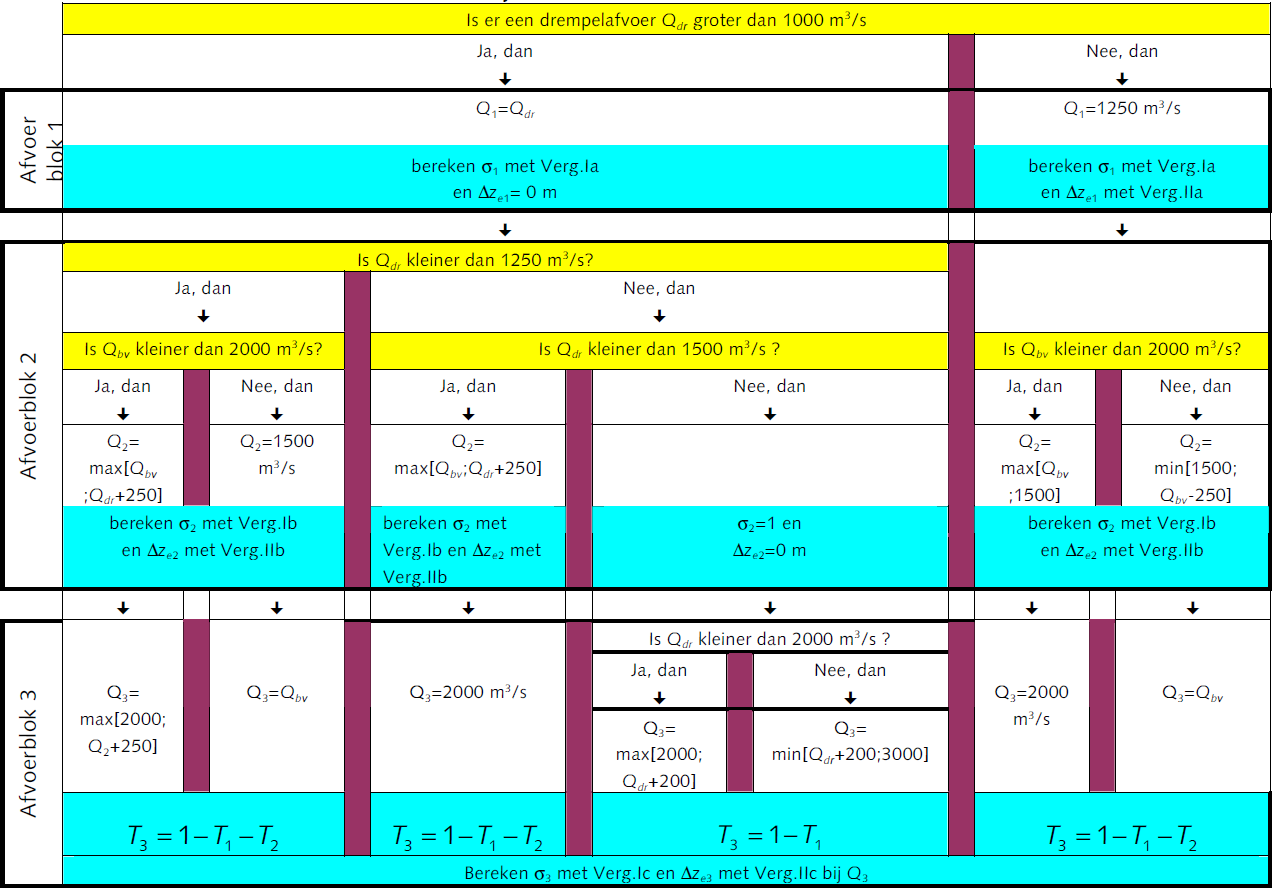
\includegraphics[width=\columnwidth]{figures/Tab8.png}
\caption{Hoofdlijn definitie afvoerblokken voor de Maas}
\label{Tab8}
\end{table}
%
\begin{equation}
\sigma_1 = e^{-\frac{w_l}{2 B_n} T_1}
\end{equation}
met $T_1 = e^{\left ( - \frac{Q_\text{stuw}}{300} \right )} - e^{\left ( - \frac{Q_1}{300} \right )}$; $Q_\text{stuw} = 100$ m\textsuperscript{3}/s en $w_l$ uit \autoref{Tab5}.
%
\begin{equation}
\sigma_2 = e^{-\frac{w_h}{2 B_n} T_2}
\end{equation}
%
\begin{equation}
\sigma_3 = e^{-\frac{w_h}{2 B_n} T_3} \text{ met $w_h$ uit \autoref{Tab8}}
\end{equation}
 met $T_2 = e^{\left ( - \frac{Q_1}{300} \right )} - e^{\left ( - \frac{Q_2}{300} \right )}$ en $w_h$ uit \autoref{Tab5}.
%
\begin{equation}
\Delta z_{1e} = -a_o \frac{q_n - q_o}{q_o}
\end{equation}
%
\begin{equation}
\Delta z_{2e} = -a_o \frac{q_n - q_o}{q_o}
\end{equation}
%
\begin{equation}
\Delta z_{3e} = -a_o \frac{q_n - q_o}{q_o}
\end{equation}
bij $Q_1$, $Q_2$ en $Q_3$ uit WAQUA.

Uitgangspunten zijn:
Bij Q=1000 m\textsuperscript{3}/s is de stroming in het zomerbed goed ontwikkeld
Bij Q=2000 m\textsuperscript{3}/s is de stroming in het zomer- en winterbed goed ontwikkeld

\section{Toepassing 1; uiterwaardverruiming met nevengeul langs de Waal}

Bij wijze van test is met Sobek de invloed van een uiterwaardverruiming met nevengeul in de Waal (km 900-905) gesimuleerd.
De nevengeul is in een 1D Rijntakkenmodel geschematiseerd als een lokale onttrekking van afvoer aan de totale rivierafvoer.
Deze onttrekking bedraagt tot 4000 m\textsuperscript{3}/s 3 \% van de rivierafvoer, daarna neemt de onttrekking lineair toe tot 10 \% bij 7000 m\textsuperscript{3}/s en blijft dit vervolgens voor nog hogere afvoeren.
Het effect op de hoofdgeul-afvoer is voor een aantal karakteristieke profielen weergegeven in \autoref{Fig7}.
De verandering in hoofdgeulafvoer die door de nevengeulen is opgewekt heeft niet het geschetste verloop van de verandering in totale rivierafvoer.
Immers, de nevengeul verlaagt ook bij lagere hoogwaterafvoeren de waterstand.
Hierdoor neemt bij een aantal profielen de \emph{afvoer door de hoofdgeul} niet evenredig af met de verruiming door de nevengeul (bv. profiel km 900,5 bij Bovenrijnafvoeren tussen de 7000 en 8000 m\textsuperscript{3}/s).

\begin{figure}
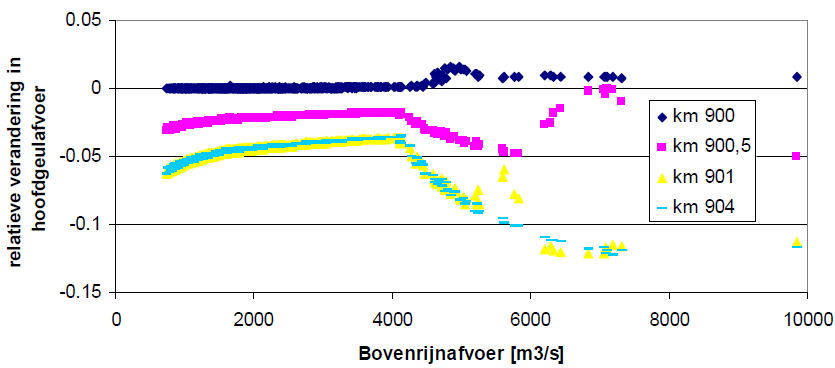
\includegraphics[width=\columnwidth]{figures/Fig7.png}
\caption{Invloed nevengeul op hoofdgeulafvoer in de Waal}
\label{Fig7}
\end{figure}

\subsubsection*{Stap 1) Karakteriseer maatregel}

De nevengeul onttrekt 3 \% van de totale afvoer voor Bovenrijnafvoeren tot 4000 m\textsuperscript{3}/s.
Daarna neemt de onttrekking lineair toe tot 10 \% bij 7000 m\textsuperscript{3}/s.
Er is geen sprake van een drempelafvoer als ondergrens voor de onttrekking.
De nevengeul is tot de rand gevuld bij een Bovenrijnafvoer van 4000 m\textsuperscript{3}/s.

\subsubsection*{Stap 2) Definitie afvoerblokken}

Omdat geen sprake van een drempelafvoer wordt voor de afvoer van het eerste blok (laagwater) Q1=3000 m\textsuperscript{3}/s gebruikt.
Voor het tweede blok (overgang tussen laag en hoogwater) geldt dat de nevengeul bij 4000 m\textsuperscript{3}/s volledig is gevuld, dus Q2=4000 m\textsuperscript{3}/s.
De afvoer Q3 van het derde blok (hoogwater) is conform het stappenplan gelijk aan 6000 m\textsuperscript{3}/s.
Hiermee kan de relatieve duur van elk blok worden bepaald volgens

\begin{itemize}
\item $Q_1=3000$ m\textsuperscript{3}/s, dan geldt $T_1 = 1-e^{\frac{800-3000}{1280}} = 0,84$
\item $Q_2=4000$ m\textsuperscript{3}/s, dan geldt $T_2 = e^{\frac{800-3000}{1280}} - e^{\frac{800-4000}{1280}} = 0,09$
\item $Q_3=6000$ m\textsuperscript{3}/s, dan geldt $T_3 = 1-T_1-T_2 = 0,07$
\end{itemize}

\subsubsection*{Stap 3) Evenwichtswaarde bodemverandering}

Voor de drie karakteristieke afvoeren is uit de Sobek resultaten voor elk relevant dwarsprofiel de evenwichtsbodemverandering bepaald volgens
%
\begin{equation}
\Delta z_{ie} = -a_o \frac{Q_{\text{hoofdgeul},n} - Q_{\text{hoofdgeul},o}}{Q_{\text{hoofdgeul},o}}
\end{equation}

\Note In het stappenplan wordt hiervoor WAQUA gebruikt voor elk rekenpunt in het zomerbed.
Deze toepassing met Sobek gebruikt echter de totale hoofdgeulafvoer en de hoofdgeul-gemiddelde diepte en geldt daarom eigenlijk slechts als verificatie van een enkele stroombaan.
De gevonden evenwichtswaarden zijn weergegeven in \autoref{Fig8}.

\begin{figure}
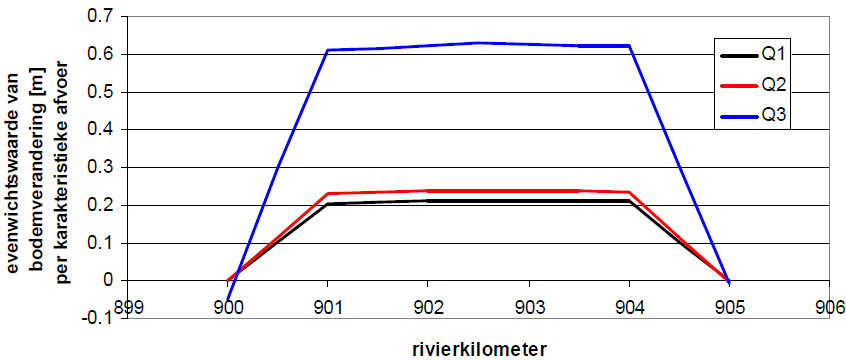
\includegraphics[width=\columnwidth]{figures/Fig8.png}
\caption{Evenwichtswaarden bodemveranderingen in de hoofdgeul, ter plekke van de nevengeul in de Waal.}
\label{Fig8}
\end{figure}

\subsubsection*{Stap 4) Bepalen tijdsfactor}

De normaalbreedte ter plekke van de nevengeul is 260 m.
De voortplantingsnelheid voor lage afvoeren bedraagt 900 m/jaar.
Voor hoge afvoeren is dit 3650 m/jaar.
Per blok kan dan worden bepaald
%
\begin{align}
\sigma_1 &= e^{-\frac{w_l}{2B_n}T_1} = e^{-\frac{900}{2 \cdot 260} 0,84} = 0,18 \\
\sigma_2 &= e^{-\frac{w_l}{2B_n}T_2} = e^{-\frac{3650}{2 \cdot 260} 0,09} = 0,73 \\
\sigma_3 &= e^{-\frac{w_l}{2B_n}T_3} = e^{-\frac{3650}{2 \cdot 260} 0,07} = 0,78
\end{align}

\subsubsection*{Stap 5) Berekenen karakteristieke bodemverandering per rekenpunt in het zomerbed.}

Met de evenwichtswaarden uit stap 3 en de tijdsfactoren uit stap 4 kunnen de karakteristieke bodemveranderingen worden berekend volgens
%
\begin{align}
z_1(0) &= [z_{1e} (1-\sigma_1) \sigma_2 \sigma_3 + z_{2e} (1-\sigma_2) \sigma_3 + z_{3e} (1-\sigma_3)]/(1 - \sigma_1 \sigma_2 \sigma_3) \\
z_2(0) &= [z_{1e} (1-\sigma_1) + z_{2e} (1-\sigma_2) \sigma_3 \sigma_1 + z_{3e} (1-\sigma_3) \sigma_1]/(1 - \sigma_1 \sigma_2 \sigma_3)
\end{align}

Ter illustratie is aanvullend aan het plan van aanpak ook de derde karakteristieke bodemverandering bepaald met
%
\begin{equation}
z_3(0) = [z_{1e} (1-\sigma_1) \sigma_2 + z_{2e} (1-\sigma_2) + z_{3e} (1-\sigma_3) \sigma_1 \sigma_2]/(1 - \sigma_1 \sigma_2 \sigma_3)
\end{equation}

Bijvoorbeeld voor dwarsprofiel km 901 geldt $\Delta z_{1e}=0,20$ m; $\Delta z_{2e}=0,23$ m; $\Delta z_{3e}=0,61$ m.
Invullen in de beide bovenstaande vergelijkingen levert dan voor km 901
%
\begin{align}
z_1(0) &= \tfrac{0,20 \cdot (1-0,18) \cdot 0,73 \cdot 0,78 + 0,23 \cdot (1-0,73) \cdot 0,78 + 0,61 \cdot (1-0,78)}{1 - 0,18 \cdot 0,73 \cdot 0,78} = 0,31 \\
z_2(0) &= \tfrac{0,20 \cdot (1-0,18) + 0,23 \cdot (1-0,73) \cdot 0,78 \cdot 0,18 + 0,61 \cdot (1-0,78) \cdot 0,18}{1 - 0,18 \cdot 0,73 \cdot 0,78} = 0,22 \\
z_3(0) &= \tfrac{0,20 \cdot (1-0,18) \cdot 0,73 + 0,23 \cdot (1-0,73) + 0,61 \cdot (1-0,78) \cdot 0,18 \cdot 0,73}{1 - 0,18 \cdot 0,73 \cdot 0,78} = 0,22
\end{align}

\subsubsection*{Stap 6) Presenteren bodemveranderingen}

Het langsprofiel van karakteristieke bodemveranderingen is samen met de door Sobek berekende waarden weergegeven in \autoref{Fig9}.
De $z_1(0)$ waarde (de grootste karakteristieke bodemverandering na perioden van grote afvoer) komt in dit geval over een met een berekende bodemverandering die gedurende 98 \% van de tijd wordt onderschreden.
De $z_2(0)$ waarde (de karakteristieke bodemverandering na perioden van lagere afvoer) komt in dit geval overeen met een berekende bodemverandering die gedurende 50 \% van de tijd wordt onderschreden.
De $z_3(0)$ waarde wijkt in dit geval nauwelijks af van $z_2(0)$, en ligt wat hoger dan de berekende 2 \% onderschreden waarde.

\begin{figure}
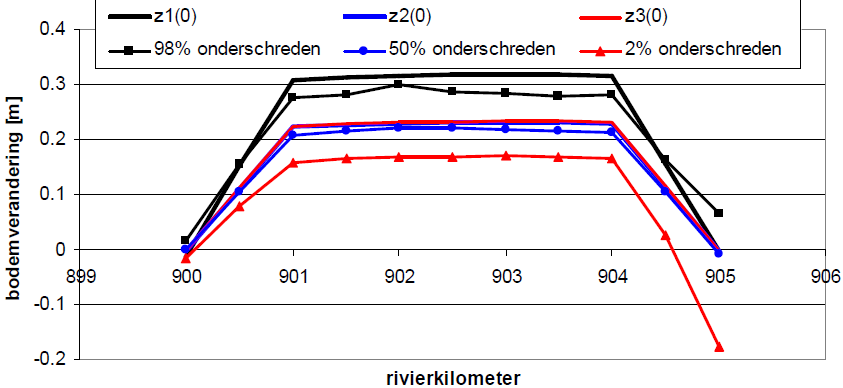
\includegraphics[width=\columnwidth]{figures/Fig9.png}
\caption{Voorspelde en berekende bodemveranderingen, ter plekke van de nevengeul in de Waal.}
\label{Fig9}
\end{figure}

\section{Toepassing 2; nevengeul langs de Lek}

De tweede test is een nevengeul langs de Lek, tussen km 930 en km 935.
Ook deze nevengeul is geschematiseerd als een lokale onttrekking van afvoer aan de totale rivier.
Deze onttrekking is opnieuw tot 4000 m\textsuperscript{3}/s 3 \% van de rivierafvoer, daarna neemt de onttrekking weer lineair toe tot 10 \% bij 7000 m\textsuperscript{3}/s en blijft dit vervolgens voor nog hogere afvoeren.
Het effect op de hoofdgeulafvoer is voor een aantal karakteristieke profielen weergegeven in \autoref{Fig10}.

\begin{figure}
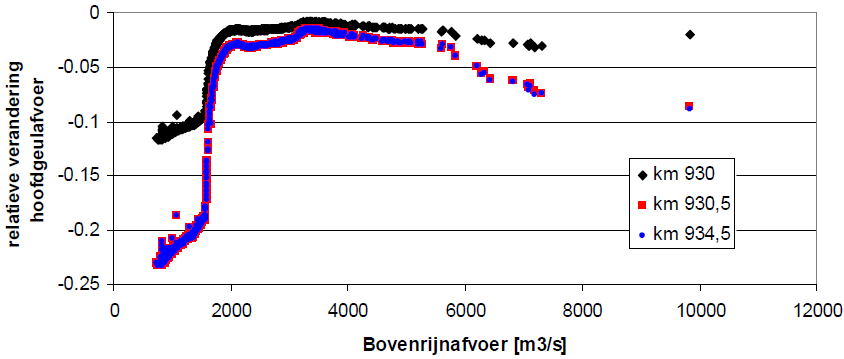
\includegraphics[width=\columnwidth]{figures/Fig10.png}
\caption{Invloed nevengeul op hoofdgeulafvoer in de Lek}
\label{Fig10}
\end{figure}

\subsubsection*{Stap 1) Karakteriseer maatregel}

De nevengeul onttrekt 3 \% van de totale afvoer voor Bovenrijnafvoeren tot 4000 m\textsuperscript{3}/s.
Daarna neemt de onttrekking lineair toe tot 10 \% bij 7000 m\textsuperscript{3}/s.
Er is geen sprake van een drempelafvoer als ondergrens voor de onttrekking.
De nevengeul is tot de rand gevuld bij een Bovenrijnafvoer van 4000 m\textsuperscript{3}/s.

\subsubsection*{Stap 2) Definitie afvoerblokken}

Omdat geen sprake van een drempelafvoer wordt voor de afvoer van het eerste blok (laagwater) Q1=1500 m\textsuperscript{3}/s gebruikt.
Voor het tweede blok (overgang tussen laag en hoogwater) geldt dat de nevengeul bij 4000 m\textsuperscript{3}/s volledig is gevuld, dus Q2=4000 m\textsuperscript{3}/s.
De afvoer Q3 van het derde blok (hoogwater) is conform het stappenplan gelijk aan 6000 m\textsuperscript{3}/s.
Hiermee kan de relatieve duur van elk blok worden bepaald volgens

\begin{itemize}
\item $Q_1=1500$ m\textsuperscript{3}/s, dan geldt $T_1 = 1-e^{\frac{800-1500}{1280}} = 0,42$
\item $Q_2=4000$ m\textsuperscript{3}/s, dan geldt $T_2 = e^{\frac{800-1500}{1280}} - e^{\frac{800-4000}{1280}} = 0,50$
\item $Q_3=6000$ m\textsuperscript{3}/s, dan geldt $T_3 = 1-T_1-T_2 = 0,08$
\end{itemize}

\subsubsection*{Stap 3) Evenwichtswaarde bodemverandering}

Voor de drie karakteristieke afvoeren is uit de Sobek resultaten voor elk relevant dwarsprofiel de evenwichtsbodemverandering bepaald volgens
%
\begin{equation}
\Delta z_{ie} = -a_o \frac{Q_{\text{hoofdgeul},n} - Q_{\text{hoofdgeul},o}}{Q_{\text{hoofdgeul},o}}
\end{equation}

\Note in het stappenplan wordt hiervoor WAQUA gebruikt voor elk rekenpunt in het zomerbed.
Deze toepassing met Sobek gebruikt echter de totale hoofdgeulafvoer en de hoofdgeul-gemiddelde diepte en geldt daarom eigenlijk slechts als verificatie van een enkele stroombaan.
De gevonden evenwichtswaarden zijn weergegeven in \autoref{Fig11}.

\begin{figure}
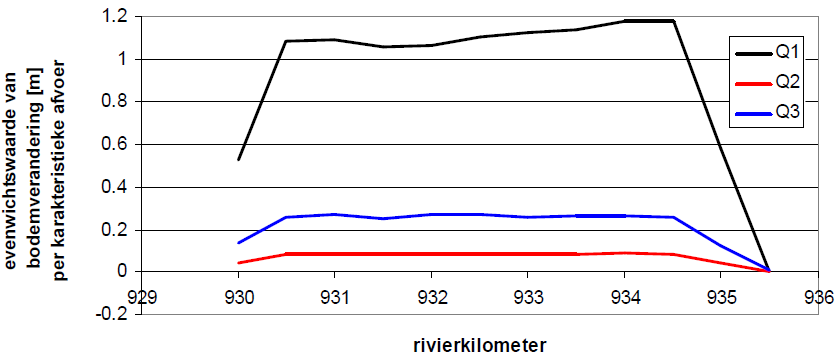
\includegraphics[width=\columnwidth]{figures/Fig11.png}
\caption{Evenwichtswaarden bodemveranderingen in de hoofdgeul, ter plekke van de nevengeul in de Lek.}
\label{Fig11}
\end{figure}

\subsubsection*{Stap 4) Bepalen tijdsfactor}

De normaalbreedte ter plekke van de nevengeul is ongeveer 140 m.
De voortplantingsnelheid voor lage afvoeren (met gesloten stuwen) bedraagt 0 km/jaar.
Voor hoge afvoeren is dit 3120 m/jaar. Per blok kan dan worden bepaald
%
\begin{align}
\sigma_1 &= e^{-\frac{w_l}{2B_n}T_1} = e^{-\frac{0}{2 \cdot 140} 0,42} = 1,00 \\
\sigma_2 &= e^{-\frac{w_l}{2B_n}T_2} = e^{-\frac{3120}{2 \cdot 140} 0,50} = 0,004 \\
\sigma_3 &= e^{-\frac{w_l}{2B_n}T_3} = e^{-\frac{3120}{2 \cdot 140} 0,08} = 0,40
\end{align}

\subsubsection*{Stap 5) Berekenen karakteristieke bodemverandering per rekenpunt in het zomerbed.}

Met de evenwichtswaarden uit stap 3 en de tijdsfactoren uit stap 4 kunnen de karakteristieke bodemveranderingen worden berekend.
Bijvoorbeeld voor dwarsprofiel km 930,5 geldt $\Delta z_{1e}=1,08$ m; $\Delta z_{2e}=0,08$ m; $\Delta z_{3e}=0,26$ m.
Invullen in de beide bovenstaande vergelijkingen levert dan bijvoorbeeld voor km 930,5
%
\begin{align}
z_1(0) &= \tfrac{1,08 \cdot (1-1,00) \cdot 0,004 \cdot 0,40 + 0,08 \cdot (1-0,004) \cdot 0,40 + 0,26 \cdot (1-0,40)}{1 - 1,00 \cdot 0,004 \cdot 0,40} = 0,20\\
z_2(0) &= \tfrac{1,08 \cdot (1-1,00) + 0,08 \cdot (1-0,004) \cdot 0,40 \cdot 1,00 + 0,26 \cdot (1-0,40) \cdot 1,00}{1 - 1,00 \cdot 0,004 \cdot 0,40} = 0,20
\end{align}

Ter illustratie is aanvullend aan het plan van aanpak ook de derde karakteristieke bodemverandering bepaald met
%
\begin{equation}
z_3(0) = \tfrac{1,08 \cdot (1-1,00) \cdot 0,004 + 0,08 \cdot (1-0,004) + 0,26 \cdot (1-0,40) \cdot 1,00 \cdot 0,004}{1 - 1,00 \cdot 0,004 \cdot 0,40} = 0,08
\end{equation}

\subsubsection*{Stap 6) Presenteren bodemveranderingen}

Het langsprofiel van karakteristieke bodemveranderingen is samen met de door Sobek berekende waarden weergegeven in \autoref{Fig12}.
De $z_1(0)$ waarde, de bodemverandering na perioden van grote afvoer komt in dit geval overeen met de $z_2(0)$ waarde, de karakteristieke bodemverandering na perioden van lagere afvoer.
De $z_2(0)$ waarde komt opnieuw overeen met een berekende bodemverandering die gedurende 50 \% van de tijd wordt onderschreden.
De $z_3(0)$ waarde komt in dit geval overeen met de berekende 2 \% waarde.

\begin{figure}
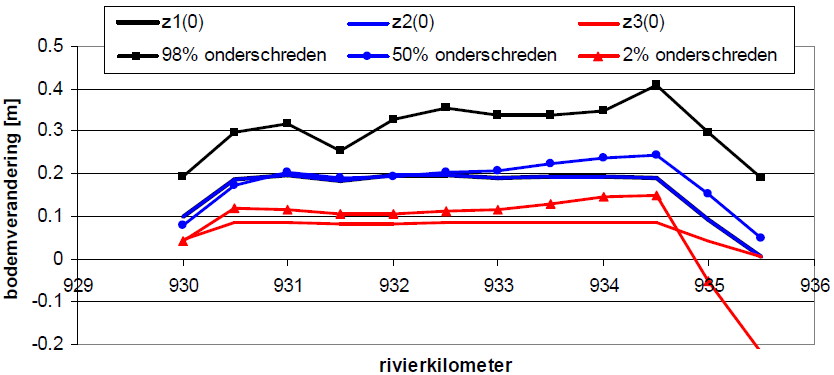
\includegraphics[width=\columnwidth]{figures/Fig12.png}
\caption{Voorspelde en berekende bodemveranderingen, ter plekke van de nevengeul in de Lek.}
\label{Fig12}
\end{figure}

\chapter{Voorbeeld toepassing Plan over de Maas}

Dit is een verslag van een pilot-toepassing van WAQMORF, een Stroomlijn-vuistregel waarmee met WAQUA resultaten een inschatting kan worden gemaakt van bodemveranderingen in het zomerbed.
Bij wijze van test is gebruik gemaakt van het WAQUA model van "Over de Maas" (WAQUA Project Over de Maas, Svasek maart 2007, nr 1426). De rekenresultaten zijn geleverd door Ed Lemaire (DLB).
De test is als volgt uitgevoerd.

\begin{enumerate}
\item Met het tooltje WAQMORF is een inschatting gemaakt van voor de morfologie representatieve berekeningen.
Dit waren de situaties bij 1250 m\textsuperscript{3}/s; 1500 m\textsuperscript{3}/s en 2000 m\textsuperscript{3}/s bij Borgharen.

\item Met deze stationaire afvoeren zijn met WAQUA plan en referentie doorgerekend waarna waterdiepten en stroomsnelheden via WAQVIEQ in export files zijn opgeslagen.

\item Met de exportfiles als invoer voor WAQMORF is een inschatting gemaakt van i) jaargemiddelde bodemverandering; ii) maximale bodemverandering (einde hoogwaterseizoen); iii) minimale bodemverandering (einde laagwaterseizoen) en iv) maximale baggerbezwaar (jaarlijks baggeren na hoogwater)
\end{enumerate}

\begin{figure}
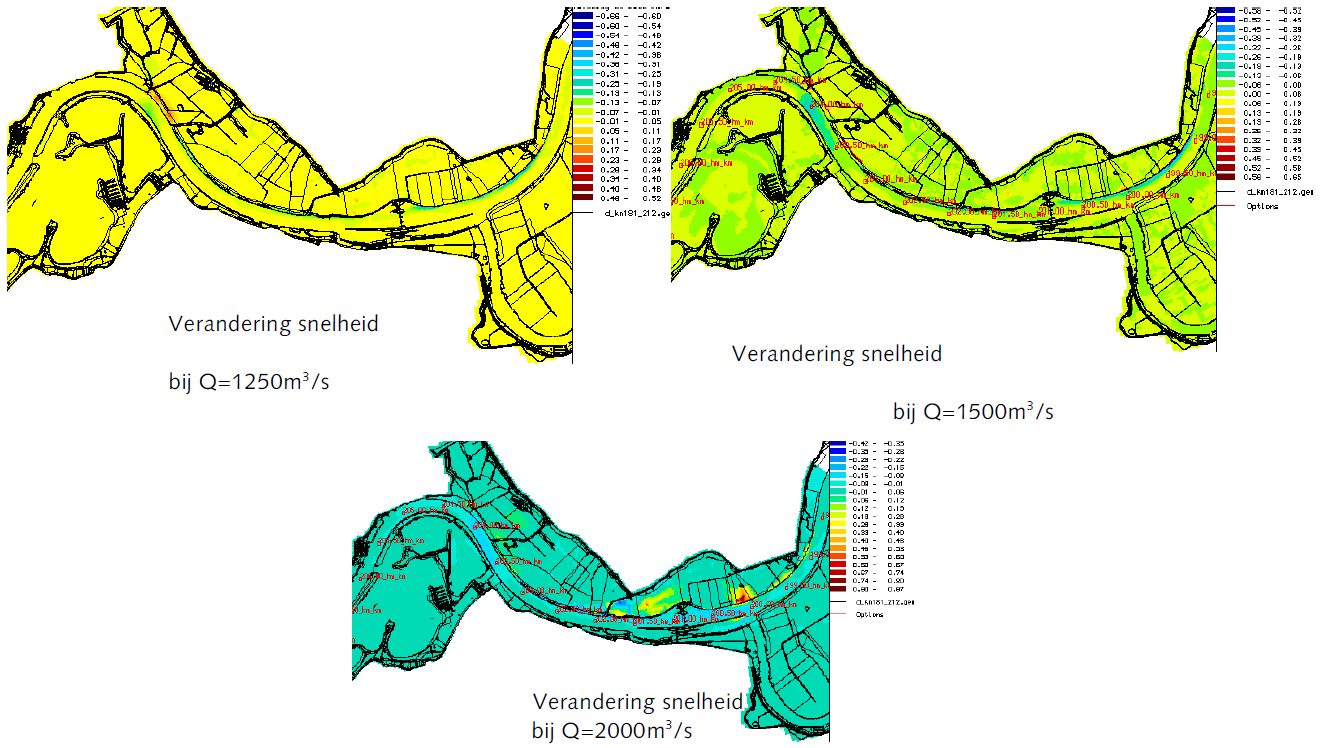
\includegraphics[width=\columnwidth]{figures/Fig13.png}
\caption{Overzicht door WAQUA berekende snelheidsveranderingen door "Over de Maas"}
\label{Fig13}
\end{figure}

De grootste lokale bodemveranderingen zijn te vinden in de bocht direct stroomafwaarts van het plan.
Bodemveranderingen zijn de jaargemiddelde waarden, weergegeven in cm.
Afhankelijk van de beschikbare ruimte in de vaargeul kan de invloed van het plan op het beheer en onderhoud van de vaargeul worden beoordeeld.

Bij wijze van test zijn drie verschillende resultaten gepresenteerd, elk voor een andere snelheids-ondergrens voor begin van beweging.
Dit heeft echter hier geen groot effect op de geschatte bodemveranderingen.

\begin{figure}
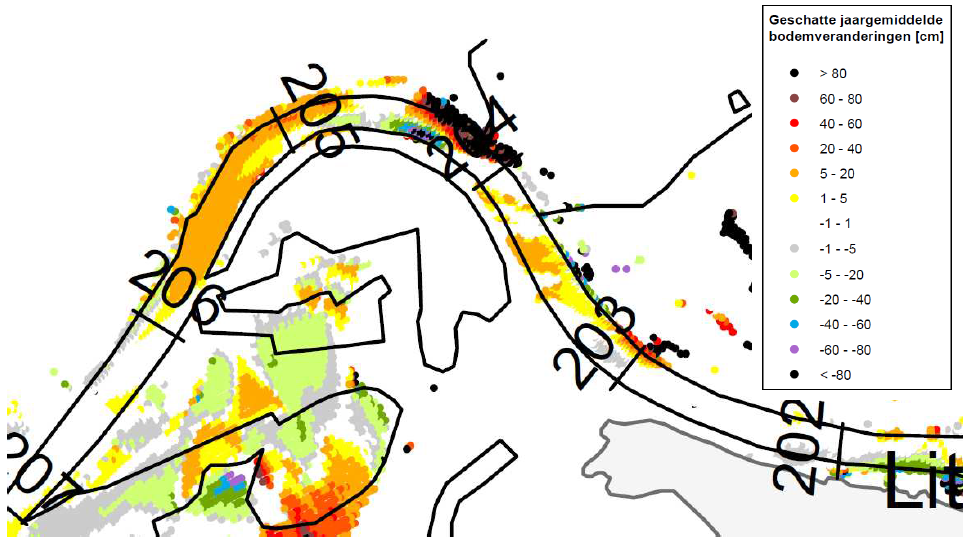
\includegraphics[width=\columnwidth]{figures/Fig14a.png}
\caption{Geschatte jaargemiddelde bodemveranderingen (ondergrens ukrit=0,01 m/s).}
\label{Fig14a}
\end{figure}

\begin{figure}
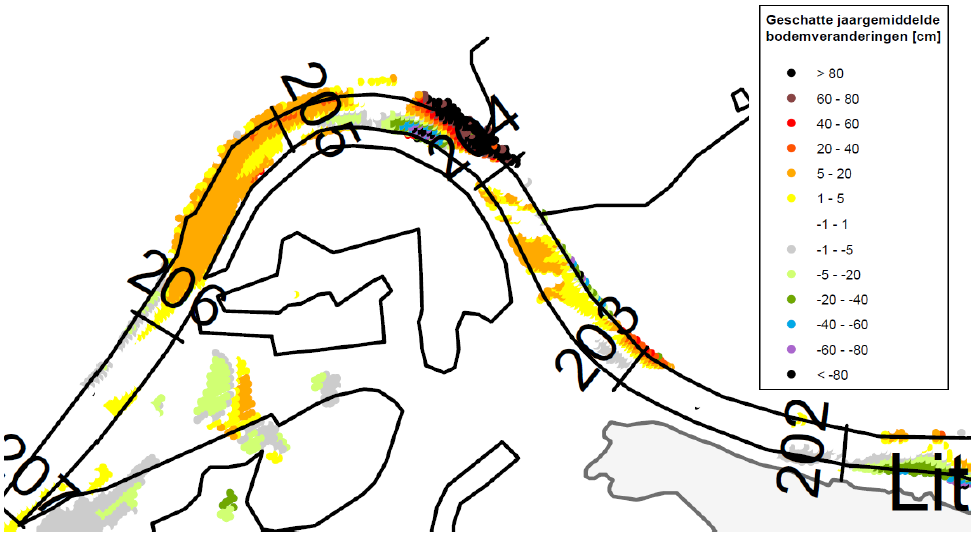
\includegraphics[width=\columnwidth]{figures/Fig14b.png}
\caption{Geschatte jaargemiddelde bodemveranderingen (ondergrens ukrit=0,10 m/s).}
\label{Fig14b}
\end{figure}

\begin{figure}
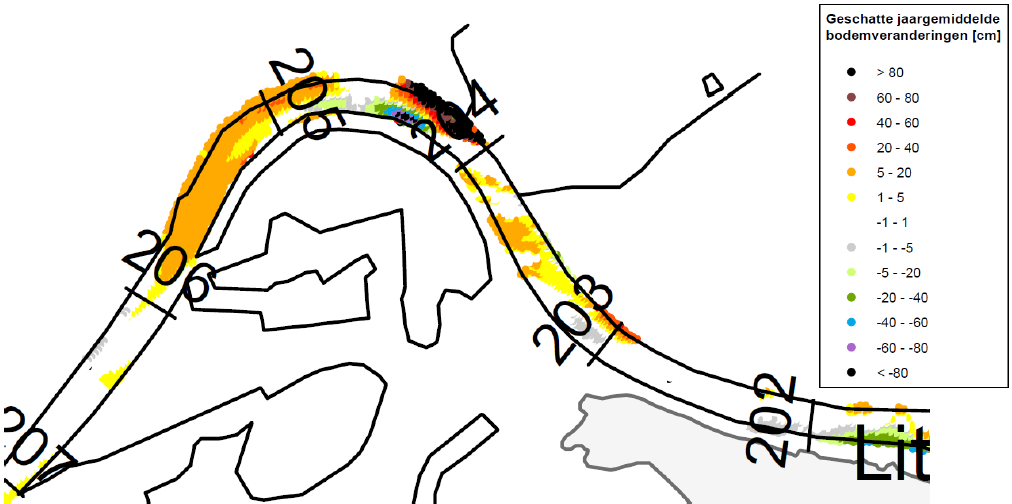
\includegraphics[width=\columnwidth]{figures/Fig14c.png}
\caption{Geschatte jaargemiddelde bodemveranderingen (ondergrens ukrit=0,30 m/s).}
\label{Fig14c}
\end{figure}

\chapter*{Referenties}

Engelund en Hansen (1967); A monograph on sedimenttransport in alluvial streams, Teknisk Forlag, Copenhagen

RIZA (2005); Morfologische effecten Ruimte voor de Rivier in het Bovenrivierengebied, werkdocument 2005.044X

Waterdienst (2008) nota Kennis en instrumenten Maas morfologie, Inventarisatie behoefte monitoring en voorspelgereedschap.